
\renewcommand{\thechapter}{4}
\chapter{Noise Measurements}
\label{ch:NoiseMeasurements}

We have described in chapter~\ref{ch:DenoisingTheory} the principles and algorithm behind denoising.  Among the points made is that a detailed noise model is required to perform denoising.  Equation~\ref{eq:FirstStatementOfNoiseCorrelations} specifies that the correlations in electronic noise will be taken as inputs to denoising; in this chapter we will describe the measurement of the noise correlations.  Section~\ref{sec:NoiseCorrelationsMath} will specify the desired measurement; section~\ref{sec:NoiseCorrelationsTimeWindows} will identify the time-dependent behavior of noise; and section~\ref{sec:NoiseCorrelationsImplementation} will describe the algorithm employed to measure noise from data.  We conclude in section~\ref{sec:NoiseCorrelationsFuture} with some possible future work to improve the quality of the noise measurements or use them in other aspects of the EXO-200 analysis.

\section{Mathematical Framework for Noise Correlations}\label{sec:NoiseCorrelationsMath}

A waveform on channel $i$ with no pulse on it consists entirely of a noise function $N_i[\tau]$.  The noise is a random function:  its value at each time $\tau$ is a random variable.  Our goal, then, is to describe the joint probability distribution of those random variables.  It has also been observed that noise on different channels is correlated, so our joint probability distribution should describe not only the noise for all time samples $\tau$ on a particular channel $i$, but also the relation between noise on any distinct pair of channels $i$ and $j$.

We can guarantee that the noise is stationary because the waveforms are all subject to shaping which removes low-frequency noise components, as described in section~\ref{sec:DetectorReadout}.  It is conventional to study stationary noise in Fourier space.  This can often lead to sharper features because noise often originates from environmental factors which demonstrate periodic behavior: in EXO-200, example of possible sources of periodic waveform noise include acoustic noise from the cleanroom, mechanical vibrations of the various wires under tension in the TPC, or switching noise from the digital power supplies.  It also can lead to a simpler characterization of noise correlations: in a steady-state environment it is impossible for noise at two different frequencies to be correlated because the $L_2$ inner product of two sinusoidal functions with different frequencies is always zero.

We will write the discrete Fourier transform of $N_i[\tau]$ as $\widetilde{N}_i[f]$, consistent with the notation described in section~\ref{sec:DenoisingNotationSetup}.  Although the specific choice of convention will not matter for any of the analysis in this work, for completeness we specify explicitly the definition of the discrete Fourier transform and its inverse as
\begin{align}
\widetilde{N}_i[f] &= \sum_{\tau = 0}^{T-1} N_i[\tau] e^{-2\pi \tau f \sqrt{-1}/T}\label{eqn:NoiseChapterDefnFourierTransform}\\
N_i[\tau] &= \frac{1}{T}\cdot \sum_{f = 0}^{T-1} \widetilde{N}_i[f] e^{2\pi \tau f \sqrt{-1}/T},
\end{align}
where $T$ is the (unitless) number of samples in the time domain waveform.  In principle both of these waveforms are periodic and extend forever; in practice we store $N[\tau]$ with $\tau \in [0, T)$ and $\widetilde{N}[f]$ with $f \in \left[0, \lfloor \frac{T}{2} \rfloor\right]$, where $\lfloor\,\rfloor$ indicates that rounding is performed downward.  This set of conventions matches the conventions of the real-to-complex discrete Fourier transform implemented by the popular FFTW library, available on all computational platforms we have attempted to use.~\cite{FFTW05}

Our sampling frequency of 1 MHz means that we can associate $\widetilde{N}_i[f]$ with noise at a frequency of $f/T$ MHz (where we again recall that $T$ and $f$ are unitless).  The accuracy of this association is dependent on the accuracy of the nominal 1 MHz sampling.  This is controlled by a nominal 80 MHz oscillator in the master TEM unit; preliminary investigations indicate that this frequency changes over time, and may deviate from a true 80 MHz period by as much as ten parts per million.~\cite{DAQWeirdDetails,EXOElectronicsFunctionalSpecification}  Since we apply low-pass filters with a combined effective cutoff frequency around 167 kHz, as described in section~\ref{sec:DetectorReadout}, this is expected to have a negligible effect on our noise measurements.

% Phase is not uniform on 2pi, since some frequency components are real-valued.  There is 180-degree symmetry, but I'm not sure how to explain this or justify why.
%We assume that the phase of the noise is random.  Since a shift in the phase of a Fourier component corresponds to a translation in the time-domain, this assumption is equivalent to assuming that waveforms are sampled at random times without any periodicity; this is certainly true for all except the solicited trigger.  The solicited trigger is taken at 10 second intervals, but the trigger time of each individual event is observed to have a root-mean-square error around 3 milliseconds.~\cite{DAQWeirdDetails}  The waveform only has a length of 2 milliseconds, so even the solicited trigger events can be assumed to have approximately random phase.  This means that the first moments of the noise, $\left<\widetilde{N}_i[f]\right>$, are all equal to zero except for the zero-frequency component $\left<\widetilde{N}_i[0]\right>$.

To quantify the second moments of the noise, we have seen in equation~\ref{eqn:SystemToSolve} that it will be useful to measure expectation values of the following real-values quantities for each pair of channels $i$, $j$ and each frequency index $f$:
\begin{subequations}\label{eq:NoiseChapterAllExpValues}\begin{align}
&\left<\widetilde{N}^R_i[f]\widetilde{N}^R_j[f]\right>\label{eq:NoiseChapterFirstExpValue}\\
&\left<\widetilde{N}^R_i[f]\widetilde{N}^I_j[f]\right>\label{eq:NoiseChapterSecondExpValue}\\
&\left<\widetilde{N}^I_i[f]\widetilde{N}^I_j[f]\right>\label{eq:NoiseChapterThirdExpValue},
\end{align}\end{subequations}
where $\widetilde{N}^R$ and $\widetilde{N}^I$ denote the real and imaginary parts of the noise in Fourier space, respectively.

We can see that equations~\ref{eq:NoiseChapterAllExpValues} possess some symmetries which may reduce the size of a file and permit the exploitation of faster matrix operations.  First, equations~\ref{eq:NoiseChapterFirstExpValue} and \ref{eq:NoiseChapterThirdExpValue} under exchange of channel indices $i$ and $j$, so we can store these values on disk more compactly by only storing the expectation values where $i \leq j$.

A second symmetry comes from the observation that for most frequencies the phase is random because an event can occur at any time and is uncorrelated with the phase of any noise frequency.  More specifically, we can decompose $\widetilde{N}[f]$ into its amplitude and phase $A[f]e^{\theta[f] \sqrt{-1}}$.  By the Nyquist-Shannon sampling theorem (see for example~\cite{659497}) we can reconstruct $A[f]$ and $\theta[f]$ this function exactly for all frequencies less than half of the sampling rate; in our case, we can reconstruct perfectly all parameters for $f < T/2$.  This means that in a waveform with odd-valued $T$ we can perfectly reconstruct all components, and in a waveform with even-valued $T$ we can perfectly reconstruct all components except $f = T/2$.  For the purpose of this section we will treat the amplitude as deterministic and only the phase as containing all of the ``randomness'' of $\widetilde{N}[f]$; this is equivalent to the assumption that high-frequency aliasing of low-frequency components (with period less than or comparable to the waveform length) is a negligible effect, or equivalently that the noise is stationary on time-scales comparable to the waveform length.  (These assumptions are only approximate, but without them we can never claim to fully measure our noise anyway, so they should not be considered extreme.)

For the frequency $f = T/2$ in an even-length time-domain waveform, we cope with this ambiguous signal reconstruction by asserting that $\theta_{T/2}$ is zero, so that the last Fourier coefficient is strictly real-valued; this comes automatically from equation~\ref{eqn:NoiseChapterDefnFourierTransform}.  Additionally, for the zero-frequency component $\theta_0 = 0$ is enforced by the fact that $N[\tau]$ is real-valued.  In all other frequency components, however, there is a unique choice of $\theta_f \in [0,2\pi)$, and it can have no directional preference because the phase of the noise and the time of the event trigger are not correlated.  Put another way, if we re-define $t' = t - t_0$ for some constant $t_0$, it will have the effect of translating all phases $\theta[f]$; our expectation values should be invariant under such an action.

We can then expand equation~\ref{eq:NoiseChapterFirstExpValue}, taking (as discussed earlier) only the phase to be random:
\begin{align}
\left<\widetilde{N}^R_i[f]\widetilde{N}^R_j[f]\right> &= A_i[f]A_j[f] cos\left(\theta_i[f]\right)cos\left(\theta_j[f]\right) \\
  &= A_i[f]A_j[f] \cdot \frac{\left<cos\left(\theta_i[f] + \theta_j[f]\right) + cos\left(\theta_i[f] - \theta_j[f]\right)\right>}{2}.\\
\intertext{We can see that $\theta_i[f] + \theta_j[f]$ is not invariant under time translation; as a result, we can assert that the left term must have an expectation value equal to zero.  On the other hand, $\theta_i[f] - \theta_j[f]$ is invariant under time translation, so that term can survive:}
\left<\widetilde{N}^R_i[f]\widetilde{N}^R_j[f]\right> &= \frac{A_i[f]A_j[f]}{2} \cdot \left<cos\left(\theta_i[f] - \theta_j[f]\right)\right>.\label{eqn:NoiseChapterPhaseEqnOne}\\
\intertext{Similarly for the other expectation values:}
\left<\widetilde{N}^R_i[f]\widetilde{N}^I_j[f]\right> &= \frac{A_i[f]A_j[f]}{2} \cdot \left<sin\left(\theta_j[f] - \theta_i[f]\right)\right>\label{eqn:NoiseChapterPhaseEqnTwo}\\
\left<\widetilde{N}^I_i[f]\widetilde{N}^I_j[f]\right> &= \frac{A_i[f]A_j[f]}{2} \cdot \left<cos\left(\theta_i[f] - \theta_j[f]\right)\right>.\label{eqn:NoiseChapterPhaseEqnThree}
\end{align}

We can see from equations~\ref{eqn:NoiseChapterPhaseEqnOne}-\ref{eqn:NoiseChapterPhaseEqnThree} that for frequencies other than $0$ and $T/2$, the following identities hold:
\begin{align}
\left<\widetilde{N}^R_i[f]\widetilde{N}^R_j[f]\right> &= \left<\widetilde{N}^I_i[f]\widetilde{N}^I_j[f]\right> \\
\left<\widetilde{N}^R_i[f]\widetilde{N}^I_j[f]\right> &= -\left<\widetilde{N}^R_j[f]\widetilde{N}^I_i[f]\right>.
\end{align}

Taking advantage of these symmetries, we can compute that for $71$ channels and waveforms containing $2048$ samples we will need to store roughly five million independent values to characterize the noise correlations; this results in a file of size roughly $40$ megabytes for each snapshot of the noise correlations.  We will show in section~\ref{sec:NoiseCorrelationsTimeWindows} that only a small number of snapshots appear to be necessary, so this can be a managable dataset.

\section{Time Windows of Constant Noise}\label{sec:NoiseCorrelationsTimeWindows}

Section~\ref{sec:NoiseCorrelationsMath} has described the renoise information which is required, and demonstrated that a snapshot of the noise will require roughly 40 MB of data.  Although EXO-200 has a significant amount of noise information available and could in principle produce a detailed history of the noise variations in time, taking such an approach would quickly produce an unmanagable quantity of data.  This section will explain how the noise behavior appears to be stable for long periods of time, permitting us to create a coarse-grained history of the noise without losing significant accuracy.

The approach to identifying these constant-noise time windows is two-fold.  Firstly, we can identify certain environmental changes which are likely to have a significant impact on the noise observed on the APDs.  Since the time at which these changes occurred is generally known precisely (and usually falls between runs), we can place time boundaries accurately when an environmental change is traced as the origin of a change.

Secondly, we develop a set of parameters which can easily be viewed in plots versus time.  These trend plots are then be reviewed qualitatively by collaboration members, and stepwise changes in any of these parameters can be taken to indicate a possible change in detector noise at this point in time.  Although sometimes it is necessary to guess the precise time when a change in noise occurred, when possible we review the environmental conditions of the detector in more detail and search for possible causes for the change in noise which would permit us to pinpoint the time of the change.

\begin{figure}
\begin{center}
\includegraphics[keepaspectratio=true,page=7,width=\textwidth,clip=true,trim=1.5in 6.8in 1.5in 1.15in]{Coherent_APD_Noise.pdf}
\end{center}
\renewcommand{\baselinestretch}{1}
\small\normalsize
\begin{quote}
\caption{Sum noise for each APD plane measured from charge injection runs, with environmental changes indicated.~\cite{JosiahCoherentAPDNoise}}
\label{fig:APDSumPlaneNoise_JosiahEnvironmental}
\end{quote}
\end{figure}
\renewcommand{\baselinestretch}{2}
\small\normalsize

\begin{figure}
\begin{center}
\includegraphics[keepaspectratio=true,page=7,width=\textwidth,clip=true,trim=1.5in 2.4in 1.5in 5.6in]{Coherent_APD_Noise.pdf}
\end{center}
\renewcommand{\baselinestretch}{1}
\small\normalsize
\begin{quote}
\caption{Sum noise for each APD electronics board measured from charge injection runs, with environmental changes indicated.~\cite{JosiahCoherentAPDNoise}}
\label{fig:APDSumBoardNoise_JosiahEnvironmental}
\end{quote}
\end{figure}
\renewcommand{\baselinestretch}{2}
\small\normalsize

\begin{figure}
\begin{center}
\includegraphics[keepaspectratio=true,page=4,width=\textwidth,clip=true,trim=1.5in 2.05in 1.5in 5.6in]{Coherent_APD_Noise.pdf}
\end{center}
\renewcommand{\baselinestretch}{1}
\small\normalsize
\begin{quote}
\caption{Sum noise for each APD pie (6-7 channels) measured from charge injection runs.~\cite{JosiahCoherentAPDNoise}}
\label{fig:APDSumPieNoise_JosiahEnvironmental}
\end{quote}
\end{figure}
\renewcommand{\baselinestretch}{2}
\small\normalsize

\begin{figure}
\begin{center}
\includegraphics[keepaspectratio=true,page=3,width=\textwidth,clip=true,trim=1.5in 6.8in 1.5in 1.15in]{Coherent_APD_Noise.pdf}
\end{center}
\renewcommand{\baselinestretch}{1}
\small\normalsize
\begin{quote}
\caption{Sum noise for all APD channels measured from charge injection runs.~\cite{JosiahCoherentAPDNoise}}
\label{fig:APDSumAllNoise_JosiahEnvironmental}
\end{quote}
\end{figure}
\renewcommand{\baselinestretch}{2}
\small\normalsize

\begin{figure}
\begin{center}
\includegraphics[keepaspectratio=true,page=6,width=\textwidth,clip=true,trim=0.2in 0.5in 0.5in 0.3in]{APD_Denoising_noise_correlations.pdf}
\end{center}
\renewcommand{\baselinestretch}{1}
\small\normalsize
\begin{quote}
\caption{Time trend of $\left<\widetilde{N}^R_{192}[385]\widetilde{N}^R_{193}[385]\right>$ (black), $\left<\widetilde{N}^R_{192}[385]\widetilde{N}^I_{193}[385]\right>$ (green), and $\left<\widetilde{N}^I_{192}[385]\widetilde{N}^I_{193}[385]\right>$ (red) corresponding to the correlations between channels 192 and 193 at 188 kHz.  Blue lines indicate tentative noise windows.~\cite{MikeCoherentAPDNoise}}
\label{fig:MikeNoise_192_193}
\end{quote}
\end{figure}
\renewcommand{\baselinestretch}{2}
\small\normalsize

\begin{figure}
\begin{center}
\includegraphics[keepaspectratio=true,page=5,width=\textwidth,clip=true,trim=0.2in 0.5in 0.5in 0.3in]{APD_Denoising_noise_correlations.pdf}
\end{center}
\renewcommand{\baselinestretch}{1}
\small\normalsize
\begin{quote}
\caption{Time trend of $\left<\widetilde{N}^R_{202}[383]\widetilde{N}^R_{203}[383]\right>$ (black), $\left<\widetilde{N}^R_{202}[383]\widetilde{N}^I_{203}[383]\right>$ (green), and $\left<\widetilde{N}^I_{202}[383]\widetilde{N}^I_{203}[383]\right>$ (red) corresponding to the correlations between channels 202 and 203 at 187 kHz.  Blue lines indicate tentative noise windows.~\cite{MikeCoherentAPDNoise}}
\label{fig:MikeNoise_202_203}
\end{quote}
\end{figure}
\renewcommand{\baselinestretch}{2}
\small\normalsize

\begin{table}
\begin{singlespace}
\begin{center}
\begin{tabular}{|c|c|p{.52\textwidth}|}\hline
Runs & Dates & Comments \\\hline
2401-2423 & 9/28/2011-9/30/2011 & APDs biased to special ``9-28-11'' settings. \\\hline
2424-2690 & 9/30/2011-11/2/2011 & FEC voltage adjustment on 11/2/2011. \\\hline
2691-2852 & 11/2/2011-11/28/2011 & Cooling fan installed on Ebox 1, 11/28/2011. \\\hline
2853-2891 & 11/28/2011-12/4/2011 & Cooling fan installed on Ebox 2, 12/4/2011. \\\hline
2892-3117 & 12/4/2011-1/13/2012 & Power outage, no data 1/13-1/19. \\\hline
3118-3326 & 1/13/2012-2/23/2012 & During runs 3314-3320 (2/22) APD channel 163 was disconnected.  During runs 3324-3331 (2/23) front-end cards were swapped.\\\hline
3327-3700 & 2/23/2012-5/11/2012 & Brief power outage on 5/11. \\\hline
3701-3933 & 5/11/2012-7/10/2012 & Possibly associated with a TEM temperature spike on the morning of 7/10; cause not known. \\\hline
3934-4003 & 7/10/2012-7/24/2012 & Possibly associated with a new TEM module on 7/24. \\\hline
4004-4126 & 7/24/2012-8/28/2012 & Power outage, no data 8/28-8/30, messy recovery of APD01. \\\hline
4127-4589 & 8/28/2012-12/27/2012 & Pump reset on 12/27, but it's not clear this is the cause of the short spike in APD noise. \\\hline
4590-4609 & 12/27/2012-1/1/2013 & As mysteriously as the noise came on 12/27, it left sometime between 1/1 and 1/2. \\\hline
4609-4779 & 1/1/2013-2/20/2013 & Not clear that anything happened on 2/20; we should review this boundary to ensure it is significant. \\\hline
4780-5061 & 2/20/2013-5/14/2013 & Noise on TPC2 changed sometime around 5/14-5/20.  Thermal stores stopped cooling on the evening of 5/17, but it it unclear how this would impact the APDs. \\\hline
5062-5197 & 5/14/2013-6/7/2013 & Modifications to electronics boards on 6/7. \\\hline
5198-5590 & 6/7/2013-8/31/2013 & Temperature excursions in the cleanroom around 8/31 permanently impacted the APD behavior. \\\hline
5591-5892 & 8/31/2013-11/11/2013 & Differential-pressure excursion on 11/11. \\\hline
\end{tabular}
\end{center}
\end{singlespace}
\caption{Recommended noise windows, based on the current understanding of changes in noise and their possible causes.  This is not the same as the noise windows actually used in the present analysis; for those, please see table~\ref{tab:NoiseWindowsUsedThisAnalysis}.}
\label{tab:NoiseWindowsRecommendedForFuture}
\end{table}

\begin{table}
\begin{singlespace}
\begin{center}
\begin{tabular}{|c|c|}\hline
Runs & Dates \\\hline
2401-2423 & 9/28/2011-9/30/2011 \\\hline
2424-2690 & 9/30/2011-11/2/2011 \\\hline
2691-2852 & 11/2/2011-11/28/2011 \\\hline
2853-2891 & 11/28/2011-12/4/2011 \\\hline
2892-3117 & 12/4/2011-1/13/2012 \\\hline
3118-3326 & 1/13/2012-2/23/2012 \\\hline
3327-3700 & 2/23/2012-5/11/2012 \\\hline
3701-3949 & 5/11/2012-7/12/2012 \\\hline
3950-4140 & 7/12/2012-9/2/2012 \\\hline
4141-4579 & 9/2/2012-12/24/2012 \\\hline
4580-4779 & 12/24/2012-2/20/2013 \\\hline
4780-5197 & 2/20/2013-6/7/2013 \\\hline
5198-5590 & 6/7/2013-8/31/2013 \\\hline
5591-5892 & 8/31/2013-11/11/2013 \\\hline
\end{tabular}
\end{center}
\end{singlespace}
\caption{Noise windows used for the current analysis.  For the noise windows recommended for future analyses and a more detailed explanation of the causes of changes in noise behavior, see table~\ref{tab:NoiseWindowsRecommendedForFuture}.}
\label{tab:NoiseWindowsUsedThisAnalysis}
\end{table}

One source of noise information is provided from charge injection runs.  These runs have been taken daily for the entire history of our dataset, and are designed to inject a known pulse half-way through the 2048-sample waveform.  Since the pulse time is known, it is also generally true that the pretrace has no signal on it and can be viewed as a pure noise sample.  It is possible by coincidence for a low-background event to deposit energy which is observed as a pulse in the pretrace, but this is extremely rare.

The approach described in~\cite{JosiahCoherentAPDNoise} is to use the pretrace samples between 200 and 800 $\mu$s from charge injection runs as noise samples.  A subset of waveforms -- APD pies, electronics boards, planes, or all APD channels together -- are summed together for each event, and the root-mean-square variation in the summed waveform is averaged over the samples between 200 and 800 $\mu$s and over all events in the charge injection run.  Each charge injection run contains 13,200 events, all of which can be used to improve the quality of this average root-mean-square measurement of noise on that subset of channels.

Figures~\ref{fig:APDSumPlaneNoise_JosiahEnvironmental} and~\ref{fig:APDSumBoardNoise_JosiahEnvironmental} show the noise for summed APD planes and electronics boards, respectively, with notable environmental changes overlaid to demonstrate their correlation with changes in noise; figures~\ref{fig:APDSumPieNoise_JosiahEnvironmental} and~\ref{fig:APDSumAllNoise_JosiahEnvironmental} illustrate the noise on APD pies and noise for all APDs summed together, respectively, without overlaid events.  These trending plots demonstrate that although the noise does undergo day-to-day fluctuations (possibly due to insufficient statistics in the charge injection runs) and some gradual changes over time, the dominant effects are from stepwise changes which are generally correlated with a change in the detector environment.

Another approach to understanding the behavior of noise with respect to time is to compute noise correlations $\left<\widetilde{N}^R_i[f]\widetilde{N}^R_j[f]\right>$, $\left<\widetilde{N}^R_i[f]\widetilde{N}^I_j[f]\right>$, and $\left<\widetilde{N}^I_i[f]\widetilde{N}^I_j[f]\right>$ for some particular channels $i$ and $j$ and frequency $f$, and identify changes in those particular values over time.  The algorithm for computing these noise correlations will be described fully in section~\ref{sec:NoiseCorrelationsImplementation}; the philosophy is simply that it is difficult to visualize changes in a dataset of five million values, but easy to visualize changes in some very small subset of those values.  We imagine that changes in the small subset may be representative of overall changes in noise behavior.

To guide this search, we focus our attention on known peaks in the noise power spectrum; furthermore, we focus on frequencies which have been observed to produce noise that is highly correlated across channels.  One example of such a noise peak is around 190 kHz, and examples of the trending of noise correlation values are shown in figures~\ref{fig:MikeNoise_192_193} and \ref{fig:MikeNoise_202_203}.  There we can see that the changes in noise correlations for a particular frequency and channel pair can be dramatic.  This method of understanding our noise seems to be a powerful and sensitive approach to complement studies based on root-mean-square noise measurements described earlier.

The currently-recommended noise run windows are listed in table~\ref{tab:NoiseWindowsRecommendedForFuture}.  Some effort has also been made to identify the reasons for changes in noise behavior, but in some cases there is no clear change to the detector that is correlated with the change in noise.  Future work may include combining all sources of noise trending information to obtain a more precise understanding of exactly when the behavior change occurred.

The run windows recommended in table~\ref{tab:NoiseWindowsRecommendedForFuture} are recommended for future work; however, they differ in some instances from the run windows used for the present analysis.  These are listed in table~\ref{tab:NoiseWindowsUsedThisAnalysis}.  In some instances the change in run range is minor and comes from a closer examination of exactly when the noise behavior changed; in others, more careful analysis revealed additional stepwise changes to the noise which had not previously been observed.  The energy resolution achieved will be shown in section~\ref{sec:RotatedEnergyResMeasurement} to be fairly stable in time, so it is not believed that the present analysis was significantly impacted by these slight variations in choice of noise run windows.

Future work can continue to improve the choice of noise run windows.  One detail which was neglected in the present analysis was selection of runs to be used within a run range.  In the present analysis, all low-background runs which were used in the final dataset were also used for noise measurements.  However, this may not always be ideal.

A specific example comes from runs 3321-3323, which occur after channel 163 was disconnected but just before electronics boards were replaced.  It is not advisable in this case for so few runs to form their own noise window because the quantity of statistics would be insufficient; but retaining them in the noise window with runs 3118-3326 could bias our estimates of noise on channel 163.  Instead, those runs should not have been used to measure noise at all; this will be corrected in future work.

Additional work may be necessary if denoising is extended to include the wire channels.  The wire noise is generally more stable than the APD noise.~\cite{JosiahCoherentAPDNoise}  However, there are exceptions to this observation; one known exception comes from the Spring of 2012, when u-wire channel 16 was mistakenly dropped from data acquisition.  If data prior to run 2464 is used in a future analysis, the change in u-wire electronics in early Fall 2011 would also need to be accounted for.

The most significant future work, though, simply consists of more careful study to characterize exactly when the noise behavior changed and whether slow changes in noise behavior may warrant the creation of additional windows.  These investigations will feed into further improvements to denoising, but they may also inform a better understanding of the noise in our detector.  The current body of work already constitutes a rich set of studies performed by many collaboration members, and has enabled the use of a manageable set of noise files for the whole history of our detector.

\section{Algorithm for Measuring Noise}\label{sec:NoiseCorrelationsImplementation}

For each of the noise windows specified in table~\ref{tab:NoiseWindowsUsedThisAnalysis}

General algorithm to create noise matrices.
Selection cuts on events.
Data format.  (Yes, this is probably useful in the category of unifying notation.)
U-wire noise collected as well, to support occasional studies.

\section{Future Directions with Noise Measurement}\label{sec:NoiseCorrelationsFuture}

Continued work on noise windows:
\begin{itemize}
\item Runs 3321-3323 should be excluded from noise measurements for the run window 3118-3326 so they don't bias our measurement of the noise on channel 163.  Channel 163 should be marked as bad in the channel map after February 22, 2012 so that it is excluded from scintillation measurements after being disconnected.
\end{itemize}

\begin{figure}
\begin{center}
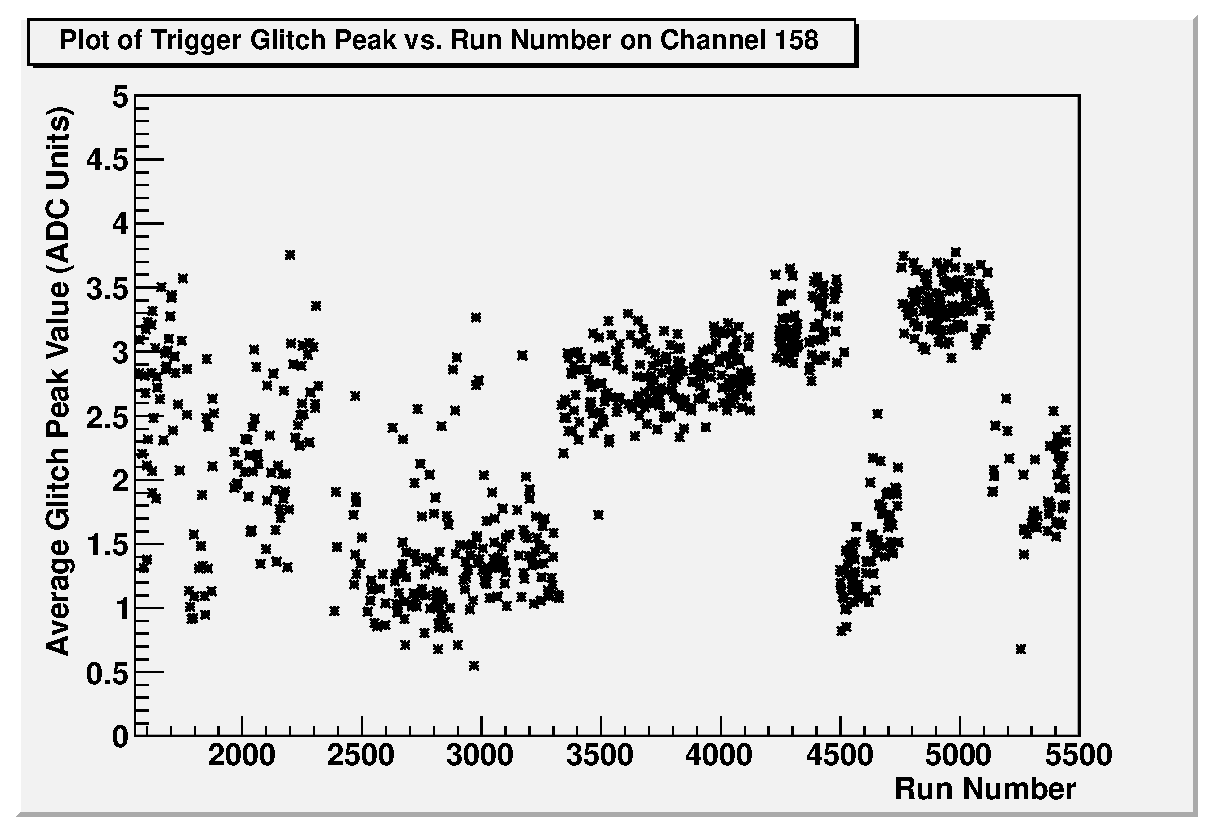
\includegraphics[keepaspectratio=true,width=\textwidth]{glitch_peak_vs_time_158.eps}
\end{center}
\renewcommand{\baselinestretch}{1}
\small\normalsize
\begin{quote}
\caption{The amplitude of the trigger-time ``glitch'' over time for channel 158.  Figure provided by Sam Homiller.}
\label{fig:GlitchPeakAmplitudeVsTime}
\end{quote}
\end{figure}
\renewcommand{\baselinestretch}{2}
\small\normalsize

stripping the glitch from noise traces.
using noise in monte carlo?
Studying the smoothness of the noise functions vs f (for truncated waveforms).
Check noise temperature dependence, other rapidly-varying environmental factors.
Resolution time-dependence can be used to check time windows; other approaches?  (KZ tests for consistency with flat.)
